Deep Memory Acquisition is a functionality that allows the Red Pitaya to set a buffer of any size for capturing signal data from the ADC. Only available for ecosystems 2.03 or newer, DMA runs at maximum ADC sampling rate of 125 MHz, writes data directly to the RAM, and relies on the AXI protocol. By default, the maximum size of the buffer (for the two input channels) is set to 2 MB, and data are saved as 32-bits per sample. According to the documentation \cite{rp}, the maximal recommended DMA region size is 412 MB for STEMlab 125-14. This amount of memory space is beyond the experimental requirement described by Equation \eqref{eq:rp_memory}. Therefore, the DMA feature seemed to fit exactly what we needed for analog input acquisition.

To get started with testing the DMA feature, the reserved memory must be reconfigured, followed by a rebuild of the device tree and restart of the Red Pitaya. I doubled the default size of the reserved memory from \texttt{0x200000} bytes $\sim$ 2 MB to \texttt{0x400000} bytes $\sim$ 4 MB. This buffer region is shared between the two channels, and the exact buffer size for each channel can be configured through programming commands.

%%%%%%%%%%%%%%%%%%%%%%%%%%%%%%%%%%%%%%%%%%%%%%%%%%%%%%%%%%%%%%%%%%%%%%%%%%%%%%%%

\paragraph{Test Acquisitions}

The Red Pitaya can be controlled remotely through SCPI (Standard Commands for Programmable Instruments) protocol available in Python and MATLAB. It can also be controlled with on-board Python and C API commands. For testing the DMA, I referenced provided examples in the official documentation and used SCPI and API commands in Python. The main code structure for both acquisitions is similar between the remote and on-board methods; it is as follows:

\begin{itemize}\setlength{\itemsep}{1pt}
    \item Configure signal units, decimation, and trigger source and level
    \item Get reserved memory region address and size
    \item Set DMA buffer address and size for each input channel
    \item Continuously acquire data until buffer is full
    \item Read data from buffer
    \item Process and save data to external file
\end{itemize}

\begin{figure}[ht]
    \centering
    \begin{subfigure}[t]{0.47\linewidth}
        \centering
        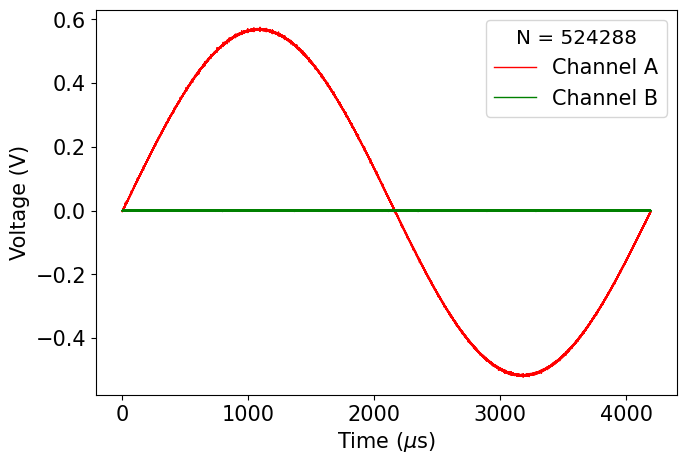
\includegraphics[width=\textwidth]{images/chapter_2/2_dma/scpi_a_v.png}
        \caption{}
        \label{fig:ch2_scpi_a_v}
    \end{subfigure}
    \hspace{.025\linewidth}
    \begin{subfigure}[t]{0.47\linewidth}
        \centering
        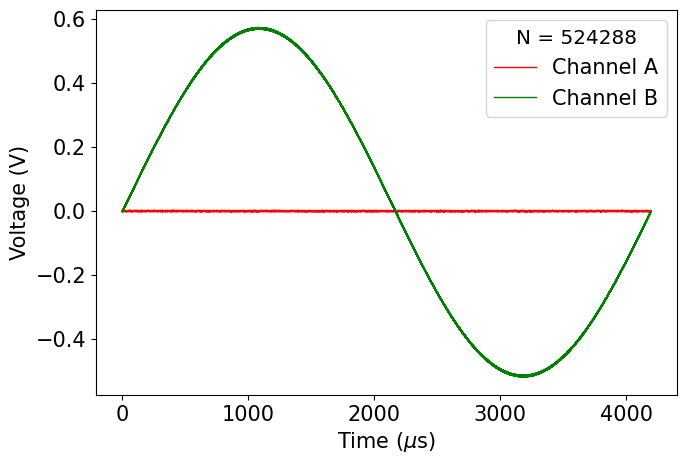
\includegraphics[width=\textwidth]{images/chapter_2/2_dma/scpi_b_v.png}
        \caption{}
        \label{fig:ch2_scpi_b_v}
    \end{subfigure}
    \caption{Input signal data acquired through DMA tests where analog signal was only connected to (a) channel A and (b) channel B. The trigger was set at the positive edge of the connected channel signal.}
    \label{fig:ch2_dma}
\end{figure}

For all tests, the reserved memory was equally distributed among the two input channels, this corresponded to 2 MB of data per channel, or 524,288 samples with each sample sizing 32 bits. Therefore, one period of an input signal at $f_\text{full}$ = 238 Hz would completely fill up the memory buffer for one channel. Figure \ref{fig:ch2_dma} shows two DMA tests using such configurations, where in each test an input signal was connected only to one channel, with the other channel unconnected. We see that the exact number of samples demanded were acquired and written to the buffer, and that precisely one period of the signal filled up the corresponding channel buffer entirely.

%%%%%%%%%%%%%%%%%%%%%%%%%%%%%%%%%%%%%%%%%%%%%%%%%%%%%%%%%%%%%%%%%%%%%%%%%%%%%%%%

\paragraph{Conclusion}

The DMA feature appears to be the most promising and powerful candidate method of analog input acquisition using the Red Pitaya that could replace the NI 5761 module in the experiment. Compared to the Streaming application, it does not present issues associated with sampling count, sampling rate, and memory overflow. However, further studies regarding Red Pitaya input noise limits and discontinuous acquisition capabilities must be explored using DMA to definitively confirm if the Red Pitaya can fully meet experimental requirements.